\chapter[\'Etude clinique]{\'Etude clinique}

Souvenons-nous brièvement de l'évolution de la signification du terme
``clinique'' enraciné dès l'Antiquité.
En s’aventurant dans les méandres de l’histoire des instruments les plus anciens comme la lyre par exemple, nous allons trouver d’abord une définition simple qui nous renseigne qu’il s’agit d’un instrument à cordes pincées, en usage dès la plus haute Antiquité, dont l’origine -selon les anciens Grecs- est faite remontée à Hermes*.
Ce dernier l’aurait construite avec la carapace d’une tortue, les cornes d’un bélier et les nerfs des bœufs soustraits à \textbf{Apollon}*, dieu de la vaticination, de la divination, \textbf{dieu archer et protecteur de la médecine, dieu des arts, en particulier de la musique}.
La musique [<gr. « mousikè » = art des Muses* qui dépendaient directement d’Apollon].
Le fameux géographe et historien grec Pausanias (2ème s. après J,-C), nous enseigne que les Muses, filles de Zeus* et de Mnémosine*, correspondaient à chacune des neuf déesses qui, dans la mythologie antique, présidaient aux arts libéraux : Clio*, la Muse de l’histoire, Calliope* (la belle voix), la Muse de l’éloquence et de la poésie épique et héroïque, Melpomène*, la Muse de la tragédie, Thalie*, la Muse de la comédie, \textbf{Euterpe*, la Muse de la musique et de la poésie lyrique} (chantée avec l’accompagnement de la lyre*, de la flûte et souvent de danse), Therpsychore*, la Muse de la danse, Erato*, la Muse de l’élégie (qui est un poème lyrique exprimant une lamentation douloureuse, des sentiments mélancoliques, donc une œuvre poétique dont le thème est la plainte), Polymnie*, la Muse de la rhétorique, du lyrisme (chant religieux et sacré, ode, poésie sacrée, caractérisée par un style élevé et hardi de l’auteur inspiré), Uranie*, la Muse de l’astronomie.
Dans un sens figuré « Muse » assume la signification de « poésie », et par extension, d’« inspiratrice » d’un poète, d’un écrivain, d’un musicien, voire ...d’un musico-thérapeute!
Homère* [< gr. = « l’aveugle » et « l’otage »], le poète mythique à qui on attribue « L’Iliade » et « L’Odyssée » (né au IXe siècle av. J.-C. à Smirne), nous fît part, à propos des Muses, du commentaire suivant : « Elles n’ont toutes qu’une seule pensée, leurs cœurs n’aspirent qu’au chant et leur esprit est dégagé de tout souci. Heureux celui qui est aimé des Muses! ».



A l’origine,\textbf{ l’activité clinique} (<gr. klinê = le lit) est celle du médecin qui, au chevet du malade, procède à l’examen des manifestations de la maladie (méthode de l’observation, de l’interrogation et de l’écoute) en vue de poser un diagnostic*, un pronostic* et une prescription* de traitement.
Michel Foucault (1926-†1984), psychologue français, dans son ouvrage capital de 1963,
«Naissance de la clinique» nous rend attentifs au fait que l’adjectif «clinique» fut longtemps du monopole médical, avec l’observation « naturelle » faite au lit du malade, uniquement à l’aide des organes sensoriels (vue, ouïe, toucher, mais aussi odorat pour l’haleine des diabétiques, le goût sucré de l’urine).
Hippocrate (médecin grec, Cos 460-377) était clinicien : il apprenait à ses étudiants l’art d’observer les symptômes, ceux-ci étant les réactions d’une personnalité à une agression pathogène. Généralisation et rationalisation, selon les critères d’Aristote, permettaient l’élaboration de « ces entités nosologiques* », les maladies, qui s’emparaient du corps du malade et poussant les médecins, exorcistes laïques, à les en faire sortir.
La « clinicité » est en régression à partir de Galien* (médecin grec, Pergame131-Rome ou Pergame, †201), au point qu’au haut Moyen Âge, le « lit du malade » devient le « lit de mort » : en effet, les personnages importants, ayant pignon sur rue et qui demandaient à se
faire baptiser seulement en fin de vie, étaient appelés – selon les dictionnaires jusqu’au milieu du XIXe siècle - « les cliniques ».
Mais c’est à Leyde (ancienne ville universitaire de Hollande), au milieu du XVIIe siècle, que réapparaît, sous forme d’une école clinique à l’hôpital, une alliance entre « la pratique et la formation enseignée », dont les effets vont diffuser en Angleterre avant de revenir sur le continent. L’expérience clinique dépassera l’ancien interdit d’Aristote, et permettra un regard scientifique sur l’individu, en incluant sa singularité sans compromettre l’objectivité.
Une des tendances communes plus manifeste dans la diversité des travaux de la psychologie semble être celle qui conduit la psychologie à l’école des faits et en particulier au comportement des malades mentaux, base sur laquelle va s’édifier la psychopathologie.
En France, l’homme qui contribue de façon décisive à l’individualisation de la psychologie pathologique, n’est pas un médecin, mais le philosophe Th. Ribot (1839-1916) qui exige la double formation de philosophie et de médecine de ses élèves (P.Janet, G. Dumas, H. Wallon, C. Blondel, G. Poyer, D. Lagache) et édifie ainsi la méthode de la psychologie pathologique. Il affirme en effet que la psychologie doit se détacher de la métaphysique en lui abandonnant l’étude des « causes premières », et doit s’attacher à l’observation scientifique des faits autrement étendus que les seules «observations intérieures »; elle peut en effet embrasser « tous les phénomènes de l’esprit chez tous les animaux, en les considérant non pas seulement sous leur forme adulte, mais dans les phases successives de leur développement.
Dans la désorganisation pathologique Th. Ribot voit un mouvement selon un ordre bien établi, d’après lequel le « nouveau » périt avant « l’ancien », ainsi que le « complexe » avant le « simple », et les différents degrés de « dissolution » réalisent pour nous une analyse des processus en leurs différents « niveaux », dont l’existence était intégrée en un fonctionnement normal. Ses publications à la Sorbonne rejoignent [avec «La psychologie des sentiments »(1896), «Les maladies de la mémoire »(1883) et «Les maladies de la personnalité » (1885)], les idées de S. Freud, montrant la primauté de la vie affective, où le tendances inconscientes jouent un rôle fondamental, et pouvant s’extérioriser soit par l’arrêt du développement affectif, soit par la dissolution des acquisitions plus récentes.
Avec l’apport de la psychologie expérimentale (en Allemagne avec
Fechner et Wundt, en France avec Claude Bernard, en Angleterre avec
Spencer et Jackson) on arrive , avec Th. Ribot, au concept de «
régression * » selon les étapes évolutives inversées : le systèmes
nerveux serait constitué de centres formant une hiérarchie : les
centres inférieurs sont les plus automatiques dans le sens que chaque centre contrôle ceux qui lui sont inférieurs et est placé sous la dépendance de ceux qui sont au dessus de lui ; les centres supérieurs sont les plus complexes et permettent les adaptations les plus différenciées, mais sont aussi les plus fragiles.
P.Janet (1859 – 1947) et G. Dumas (1866-1946), élèves de Ribot, fondèrent ensemble en 1904 « Le journal de psychologie normale et pathologique », et leurs œuvres contiennent l’idée de privilégier l’observation des « conduites » ayant une signification et un but.
Dumas consacre lui aussi beaucoup d’attention à «L’étude des émotions», aux « Troubles mentaux et de guerre » et dirige la publication d’un « Traité de Psychologie » (1923-1930).
L’expression « psychologie clinique » apparaît sous la plume de S. Freud, dans sa lettre à W. Fliess du 30.01.1899 : « Maintenant, la connexion avec la psychologie, telle qu’elle se présente sur les Etudes sur l’hystérie(1895) sort du chaos, j’aperçois les relations avec le conflit, la vie, tout ce que j’aimerais appeler psychologie clinique ».Dès 1896, le psychologue américain Lightner Witmer (1867-1956) avait ouvert en Pennsylvanie une Psychological Clinic destinée aux enfants retardés et anormaux et avait forgé l’expression de « méthode clinique en psychologie ».
A Paris, de décembre 1897 à décembre 1901, on assiste à la publication de la « Revue de psychologie clinique et thérapeutique » (six numéros par an, sous la direction de Valentin et Hartenberg), dont les intentions s’avèrent prémonitoires, et dont l’utilisation de l’expression « psychologie clinique » paraît pionnière.
L’approche de Janet (cf. supra) ne manque pas de lier la clinique psychologique à la pratique médicale, dans le sens de connaître les troubles afin de pouvoir les soulager, la psychologie clinique étant l’application à la médecine des découvertes expérimentales.
En effet, tout en puisant dans la recherche de laboratoire de précieux renseignements, elle observe la vie psychologique elle-même, considérée comme un tout concret et réel, réunissant dans une vue d’ensemble les réactions naturelles et spontanées du sujet, en présence des excitations de tout genre, qui exprime son tempérament et porte la marque de son caractère. Par les influences de l’hérédité et du milieu, elle poursuit le développement, normal et pathologique de la personnalité, la tâche n’étant pas de schématiser, mais d’individualiser.
Plus tard, le défi lancé par la psychologie clinique, comportera la singularité des patients (avec son intériorité subjective) à concilier avec la rigueur scientifique, chose qui a été promue , pendant l’éclosion du structuralisme (1949 – 1974), par des personnalités comme Daniel Lagache et Juliette Favez-Boutonier.
La totalité d’une personnalité est singulière parce qu’elle est éminemment complexe, et la relation thérapeutique n’est rien d’autre que Amour, l’amitié, le besoin de société, et tous les sentiments sociaux sont évidemment composés par une foule d’éléments divers.
Dès 1938, Lagache parle d’une « psychologie nouvelle» devenue fonctionnelle, et non plus seulement structurale, décrivant l’homme en situation, et faisant du conflit (dimension plus « dramatique » de l’existence humaine) la condition nécessaire de la prise de conscience.
Le conflit n’est pas représenté comme un nœud dans l’inconscient, mais comme la dynamique d’une prise de conscience.
En voie de « définition », la psychologie clinique s’intéresse moins
aux tests et plus aux à-côtés des tests, c. à d. aux réactions de la
personnalité à la situation à la fois matérielle et sociale dans
laquelle le sujet se trouve placé. L’expérience de la recherche et de
l’enseignement nous a montré la fécondité de cet envisagement qui
n’est pas autre chose que l’application de la méthode clinique à
l’homme total ; ceci n’implique pas un renoncement à l’expérimentation
ou à la mesure de certaines aptitudes spéciales ou même de
l’efficience intellectuelle, seulement, l’épreuve spéciale analytique, quantitative, ne prend tout son sens que rapprochée d’autres épreuves analogues (comme dans le profil psychologique) intégrée dans le portrait psychologique global.
Cette réciprocité de l’ensemble et du détail est une condition générale de la psychologie humaine : sur l’intuition d’ensemble initiale quelques faits particuliers viennent se profiler, l’image de l’ensemble est révisé et permet d’interpréter de nouveaux détails ; d’autres détails modifient à nouveau l’ensemble, et ainsi de suite-
L’analogie est frappante avec la médecine clinique : là aussi on a espéré substituer à l’art clinique incertain une somme d’examens de laboratoire ; mais là aussi il a fallu revenir à l’idée d’une intégration des examens de laboratoire dans l’ensemble clinique.
L’ « investigation » (terme cher à Lagache) la plus poussée n’a pas comme but une analyse destructrice et méchante, mais une connaissance ouverte et édificatrice de la personne. Quel savoir pour une pratique clinique ? Ce qui caractérise la psychologie clinique c’est justement la méthode clinique c’est à dire la nature des opérations avec lesquelles le psychologue clinicien approche la conduite humaine :1. L’examen historique exhaustif, aboutissant à un tableau du cas à partir duquel il sera construit un cheminement et des hypothèses diagnostiques, suivies d’un pronostic nuancé.
2. L’observation longitudinale : entretiens réguliers à long terme (de plusieurs mois) : étude des conduites, des conditions de maturation, l’hérédité, les conditions psychopathologiques etc
3. L’examen par des tests standardisés (niveau intellectuel, cognitif etc) en f(x) des groupes d’âge ; la construction d’un « profil » en fonction de la théorie sous-jacente aux tests ; un pronostic « nuancé » sous forme numérique.
4. L’examen de personnalité par la méthode projective (Rorschach, Tat, Cat, Szondi etc), sur la base d’un matériel perceptif parfois très peu structuré, resté inchangé depuis le début de leur application ~1930, et dont la compréhension repose sur la théorie psychanalytique.
5. L’apport de la perspective interactionnelle (systémique) :
-les interactions familiales, horizontales, verticales , obliques, intra ou extra famille restreinte (famille élargie ou entourage), génogramme,
-les interactions sociales, scolaires, professionnelles, extra- professionnelles, -les appartenances (mythes familiaux, religion, culture etc),
-les interactions groupales (volées d’écoles, évent. Groupes de discussion ou
de psychothérapie etc).
L’objet de la psychologie clinique (D. Lagache)
La définition « officielle » de la psychologie clinique mobilise et articule la singularité et
la totalité, de façon à reconnaître une discipline psychologique basée sur l’étude approfondie des cas individuels, l’étude de la conduite humaine individuelle et de ses conditions (hérédité, maturation, conditions psychologiques et pathologiques, histoire de la vie), en somme, l’étude de la personne totale «en situation», c.àd. l’expérience vécue de ce rapport à l’environnement.
Les buts : conseiller, guérir, éduquer (ou rééduquer par la psychopédagogie clinique), voir prévenir et résoudre un conflit. La prévention (surtout de la délinquance et de la criminalité) est liée à la vocation à travailler dans des situations concrètes, avec les travailleurs sociaux.
Si le psychanalyste peut choisir de ne se préoccuper que du conflit intra-psychique, le clinicien est, quant à lui, fondé à prendre en charge le conflit externe, puis à faire la synthèse des deux dimensions conflictuelles.
Le diagnostic est l’acte cognitif caractéristique de l’approche clinique et correspond à l’acte essentiel de la psychologie clinique: il s’agit de ramener le cas individuel à des relations générales empruntées au savoir théorique.
Les moyens correspondent à l’examen psychologique qui comporte - comme investigation de la conduite – la conduite extérieure manifeste, l’expérience consciente (par le récit du consultant, y compris les modifications somatiques subjectives), les modifications somatiques objectives (physiologie), les produits de la conduite (écrits, dessins, travaux manuels, performances aux tests), etc.
Les techniques, au nombre de cinq, sont, les techniques historiques (technique testimoniale et documentaire), les techniques d’observation (examen clinique proprement dit, observation continue), emploi des tests (psychométriques, de niveau, d’aptitudes, de personnalité, projectifs), techniques auxiliaires (morphologie, graphologie), techniques psychanalytiques (investigations psychanalytiques).

Au vue de cet aperçu historique, on peut reconnaître que
dans certains milieux psychiatriques actuels, la musicothérapie trouve
plus sa place aussi dans le complètement des tableaux cliniques.

Dans notre étude, l'axe principal porte sur la
vérification de l'amélioration de
la capacité d'écoute suite au travail musicothérapeutique.

\section{Cadre de travail, population}

 La clinique privée (Privatklinik)
de Meiringen (BE) est  principalement spécialisée en
addictologie avec problèmes d'alcool et de toxicodépendance, couvrant aussi les aspects dépressifs
et les
burnouts.


Elle dispose d'une capacité de 195 lits, et le temps de séjour fluctue de 3 à 6 semaines ou plus, en
fonction de la participation des assurances.

Actuellement, en plus de l'administration et l'intendance, les 33
médecins et psychiatres, sont
accompagnés par 177
soignants, dont infirmiers psychiatriques, aide-infirmières, physio et
ergothérapeutes, 
psychologues et intervenants en \textit{thérapies
créatives }, comme l'art-thérapie, thérapie
corporelle, zoothérapie (chien/cheval),  ateliers de créativité --
bois et terre --,  les textiles et la\textbf{ musicothérapie} avec deux
personnes, dont la souscrite à titre de 10 pour cent.


%\textbf{Organigramme}: nous avons obtenu l'autorisation de vous
%montrer l'organigramme de la Clinique de Meiringen lors de la
%soutenance.




%(-OH*:  le radical hydroxile, oxydrile de la molécule éthylique)




L'\textbf{échantillonnage} fortement conditionné par les contraintes
institutionnelles, comme les interruptions prématurées de séjour, les rendez-vous
 médicaux superposés, l'impossibilité de participation physique et/ou
 psychique, les remplacements disparates et hétéroclites de ma
 collègue, l'emploi à
 temps partiel, a été restreint  par le choix d'un nombre limité de
 patients (Nb=29).
Une autre contrainte de nature extra-institutionnelle allant dans le
même sens réside dans l'éloignement géographique.

En synthèse:
 \begin{itemize}
 
 \item \textbf{Nombre total de personnes}: Nb= 29 
\item\textbf{Genre et âge de la population étudiée:}  19 hommes et 10 femmes, de 25 à 72
  ans dont l'âge moyen est de 48 ans. x= 48.
 \item\textbf{Pathologies}: burnout, dépendances, dépression.
 \item \textbf{Nombre total de séances} par personne en
   musicothérapie= 4 ;   \textbf{mu}=1/semaine;  
 \textbf{t}= 50--60 min, période = 3 -- 4 semaines.
\end{itemize}




 %mu en grec
\section{Méthodologie et  ensemble des démarches}
Obtenu l'aval de la direction de la
clinique pour cette étude,  le personnel soignant et l'ensemble des
thérapeutes (ateliers, thérapies créatives, kynési--cyno--
et hippothérapie) vont être informés aussi par écrit.

Le même texte, destiné de même aux
patients\footnote{ \emph{Information für Mitwirkende an der klinischen
  Studie\  ``Evaluierung des aktiven Hörvermögens" //Cf.Annexe D}
}, explique le projet de l'étude sur l'écoute, comme aussi la transformation
avec ou sans musicothérapie.
Le consentement libre est validé par la signature du patient, après
un court entretien avec lecture du texte\footnote{\emph{``Eine schriftliche Einbewilligung zum
    Test"}.}, assuré par  Regula Lehman.\footnote{Regula
  Lehmann, musicothérapeute  à 90\%  à la clinique de Meiringen.} 


Après ces prémisses, l'étude commence véritablement avec l'application du test
audiométrique suivie du questionnaire qualitatif.

\textbf{L'étude }est
réalisée en fonction des séjours variables des patients, soit une
totalité  de quatre semaines
distribuées dans l'intervalle juin --
octobre 2017,  à l'aide de tests et questionnaires appliqués en début
et fin de séjour.

\textbf{Types de thérapie, musicothérapie} réceptive et/ou active.
Les autres formes de thérapies, en gardant
leur indépendance par rapport à notre analyse, se déroulent simultanément, à
l'exception de la musicothérapie pour le groupe contrôle.

L'utilisation particulière du \textit{test de perception d'écoute de Tomatis}  est
légitimée par sa facilité et  simplicité d'application, en dehors de
son contexte thérapeutique.






\textbf{Le Groupe Musicothérapeutique (expérimental) GM} comporte 21
patients, dont 6
femmes et 15 hommes.


\textbf{Le  Groupe Contrôle GC} comporte 8 patients, dont 4 femmes et 4 hommes.


Le nombre
des patients s'est limité  à 8
patients (4 hommes/4 femmes) pour le GM, et à 7 patients (4 hommes/3
femmes) pour le GC pour obtenir une comparaison entre les tests et les questionnaires.




Compte tenu de ce que nous avons considéré, nous ------
 Après avoir décrit largement plus haut le test d'écoute, il est nécessaire d'apporter aussi des compléments d'informations sur le WHO QOL-Bref. Il a été
 utilisé ici en parallèle pour constater s'il y a une transformation sujective psychique du sujet,
 positive ou négative.
\textbf{ Les instruments de mesure}: le test  d'écoute et le WHO QOL

 \subsection{Le WHO QOL - Bref:  World Health
   Organisation Quality of Life Assessement }
 Le  WHOQOL-Bref sert à évaluer la qualité de vie des patients. C'est une échelle
d'auto-évaluation subjective qui évalue la santé mentale, le
bien-être, l'environnement et les relations sociales.
Il s'agit ici de la version courte  la plus récente (2004) du questionnaire
 WHOQOL-100 datant de 1998, version issue du Programme sur la santé
 mentale de l'
Organisation mondiale de la santé de Genève. Il y a 26 questions
courtes, dont un item concernant la qualité de vie globale
auto-évaluée par le sujet, un item évaluant la santé générale perçue
et les 24 autres se répartissent selon les 4 domaines suivants:  
: physique, psychologique, relations sociales et environnement.
\begin{enumerate}
\item  Le domaine de la perception physique (7 items) comprend l' activité quotidienne// la dépendance et/ou l'assistance médicale// la fatigabilité, l'énergie//la mobilité// la douleur// le sommeil// la capacité de travail//
	
\item Le domaine psychologique (6 items):  image de soi, apparence// ressentis positifs et négatifs// estime de soi// spiritualité, croyances personnelles, religion// mémoire et concentration, apprentissage, pensée.
		
\item Le domaine des relations sociales (3 items) : relations personnelles// soutien social// vie sexuelle.
			
\item Le domaine de l'environnement (8 items) :
                         l'environnement domestique et physique
                         (pollution, bruit, trafic, climat)// la
                         situation financière//  la liberté, la
                         sécurité physique et morale//
                         l'accessibilité et qualité de la santé// les
                         opportunités de détente, loisirs, accès aux
                         informations// logement et transport// 
\end{enumerate}
		
	

Les questions varient selon sa propre perception, telle la satisfaction
au sujet de son  sommeil, de sa vie relationelle, sexuelle, de
l'opinion de que l'on a sur soi,  `` Êtes-vous satisfait de
vous-même?'' , ``Acceptez-vous votre apparence physique?''ou si le patient éprouve souvent des sentiments négatifs
et/ou s'il a assez d'énergie dans la vie de tous les jours.
La cotation se fait sur 4 types d'échelles de réponses en 5 points (de 1 à 5)
permettant l'évaluation de l'intensité, la fréquence, la capacité, l'évaluation.

Le patient le remplit avec ou sans aide du
thérapeute lors de chaque test
d'écoute. La durée variera de 3 à 10 minutes en
moyenne. 
Nous avons utilisé et fait en parallèle le test WHOQO-Bref pour avoir une variable supplémentaire pour confirmer en
parallèle supposée de l'action de la musicothérapie sur une éventuelle modification de l'écoute.


        	
 \subsection{Technique d'intervention:}


       
\begin{itemize}
\item Le groupe GM avec musicothérapie : un
          test avant leur prise en charge en musicothérapie; avec un questionnaire
          WHOQOL.
          
\item Un 2\ieme\ test et un questionnaire WHOQOL : après 4 semaines de
          clinique.
          
\item Un groupe GC sans musicothérapie, (contexte idem)
	toujours dans le même contexte, c.à.dire en clinique, avec le suivi et les mêmes protocoles que l'autre groupe. Un premier test avant
        puis un deuxième test, avec les questionnaires WHOQOL, après 4 semaines.
        
\end{itemize}

\textbf{ Par ordre chronologique:}
 
\begin{enumerate} 
   \item Un test d'écoute, un entretien et un questionnaire
        WHOQOL pour les deux groupes.
    \item Séances de musicothérapie, actives ou réceptives (1x par
        semaine) pour GM.
    \item Deuxième test d'écoute, entretien et questionnaire
      WHOQOL pour les deux groupes.
      
\end{enumerate}

	
	
	\textbf{Durée des tests} : Chaque test d'écoute a une durée  moyenne de
        70 à 90 minutes par patient. Pour chacun, nous avons donc réalisé
        en tout 2h30 de tests d'écoute sur lesquels
        s'ajoute un court 
t        entretien (2x10').

        
        Le questionnaire WHOQOL (2x10')  a été remplis par les
        patients avant le début du séjour en clinique et après, lors
        de leur sortie, sans aide.
        
       
      
      \paragraph{Résultats, nombre de tests et questionnaires GM et GC:}

       
     Nous avons réalisé en tout pour GC et GM \textbf{44 tests d'écoute et 25 questionnaires 
     WHOQOL-Bref.}
     
     \textbf{Les tests d'écoute}: il y a\textbf{ 30 tests d'écoute } valides qui serviront de
     comparatif (1°+2°= avant/après).
     
\textbf{Pour le GM}:
     
     21 personnes ont fait le 1°test et 8 d'entre-elles ont fait le
     2°test.

     Nous allons extraire les données de 8 personnes avec 2 tests (avant/après), soit  un
     total de \textbf{16 tests d'écoute } pour le groupe
     d'expérimentation, en musicothérapie.

     
     1°: GM= 21
    
     2°: GM= 8
     
     \textbf{ Pour le GC}:

     
     8 personnes ont fait le 1°test et 7 le 2°.
     
\paragraph{Déroulement de l'étude:}


     1°: GC= 8

     2°: GC= 7
     
     Nous avons un total de \textbf{14 tests d'écoute} valides pour le
     comparatif.

     
Total des 2 groupes réunis:\textbf{ 30 tests d'écoute}.
     


\textbf{Les questionnaires WHOQOL}: 25

     \textbf{Pour le GM}:      
     10 questionnaires (8x1°) et (2x2°) pour GM.
     
     1°: GM= 8 

     
     2°: GM= 2
   
     
\textbf{ Pour le GC}:
15 questionnaires (8x1°) et (7x2°) pour GC.
    
     1° GC= 8
     
     2°: GC= 7
     
     Nous avons un total de \textbf{7 questionnaires} valides pour le
     comparatif.
     
Total des 2 groupes réunis:\textbf{9 questionnaires}.
    
 
     
          
 
 
 	
 	
       

 	
 	\section{Déroulement de l'étude avec un groupe
          de contrôle et un groupe d'intervention}





                                      Patients souffrant de dépression, burnout
                                               en séjour dans la
                                               clinique, répartis en
                                               deux groupes.
                                               Nous avons conscience
                                               d'avoir mélangé deux
                                               symptomatologies qui
                                               toutefois paraissent
                                               sous-tendues par les
                                               mêmes mécanismes et
                                               s'exprimant par une
                                               humeur négative.

\begin{figure}
\centering
\includegraphics[width=0.7\linewidth]{images/Groupecontrole.png}
\caption[Schéma du déroulement]{Déroulement de l'étude avec GM et GC}
       
\label{groupecontroleimage1}
\end{figure}
\textbf{Un test type dépressif}: 
En guise de préambule, la figure 6.2. illustre l'exemple type du test
d'écoute d'un sujet dépressif réalisé lors de notre
étude en clinique: la
chute des fréquences dans des zones de fréquences élevées est
clairement visible.
 \begin{figure}
	\centering
	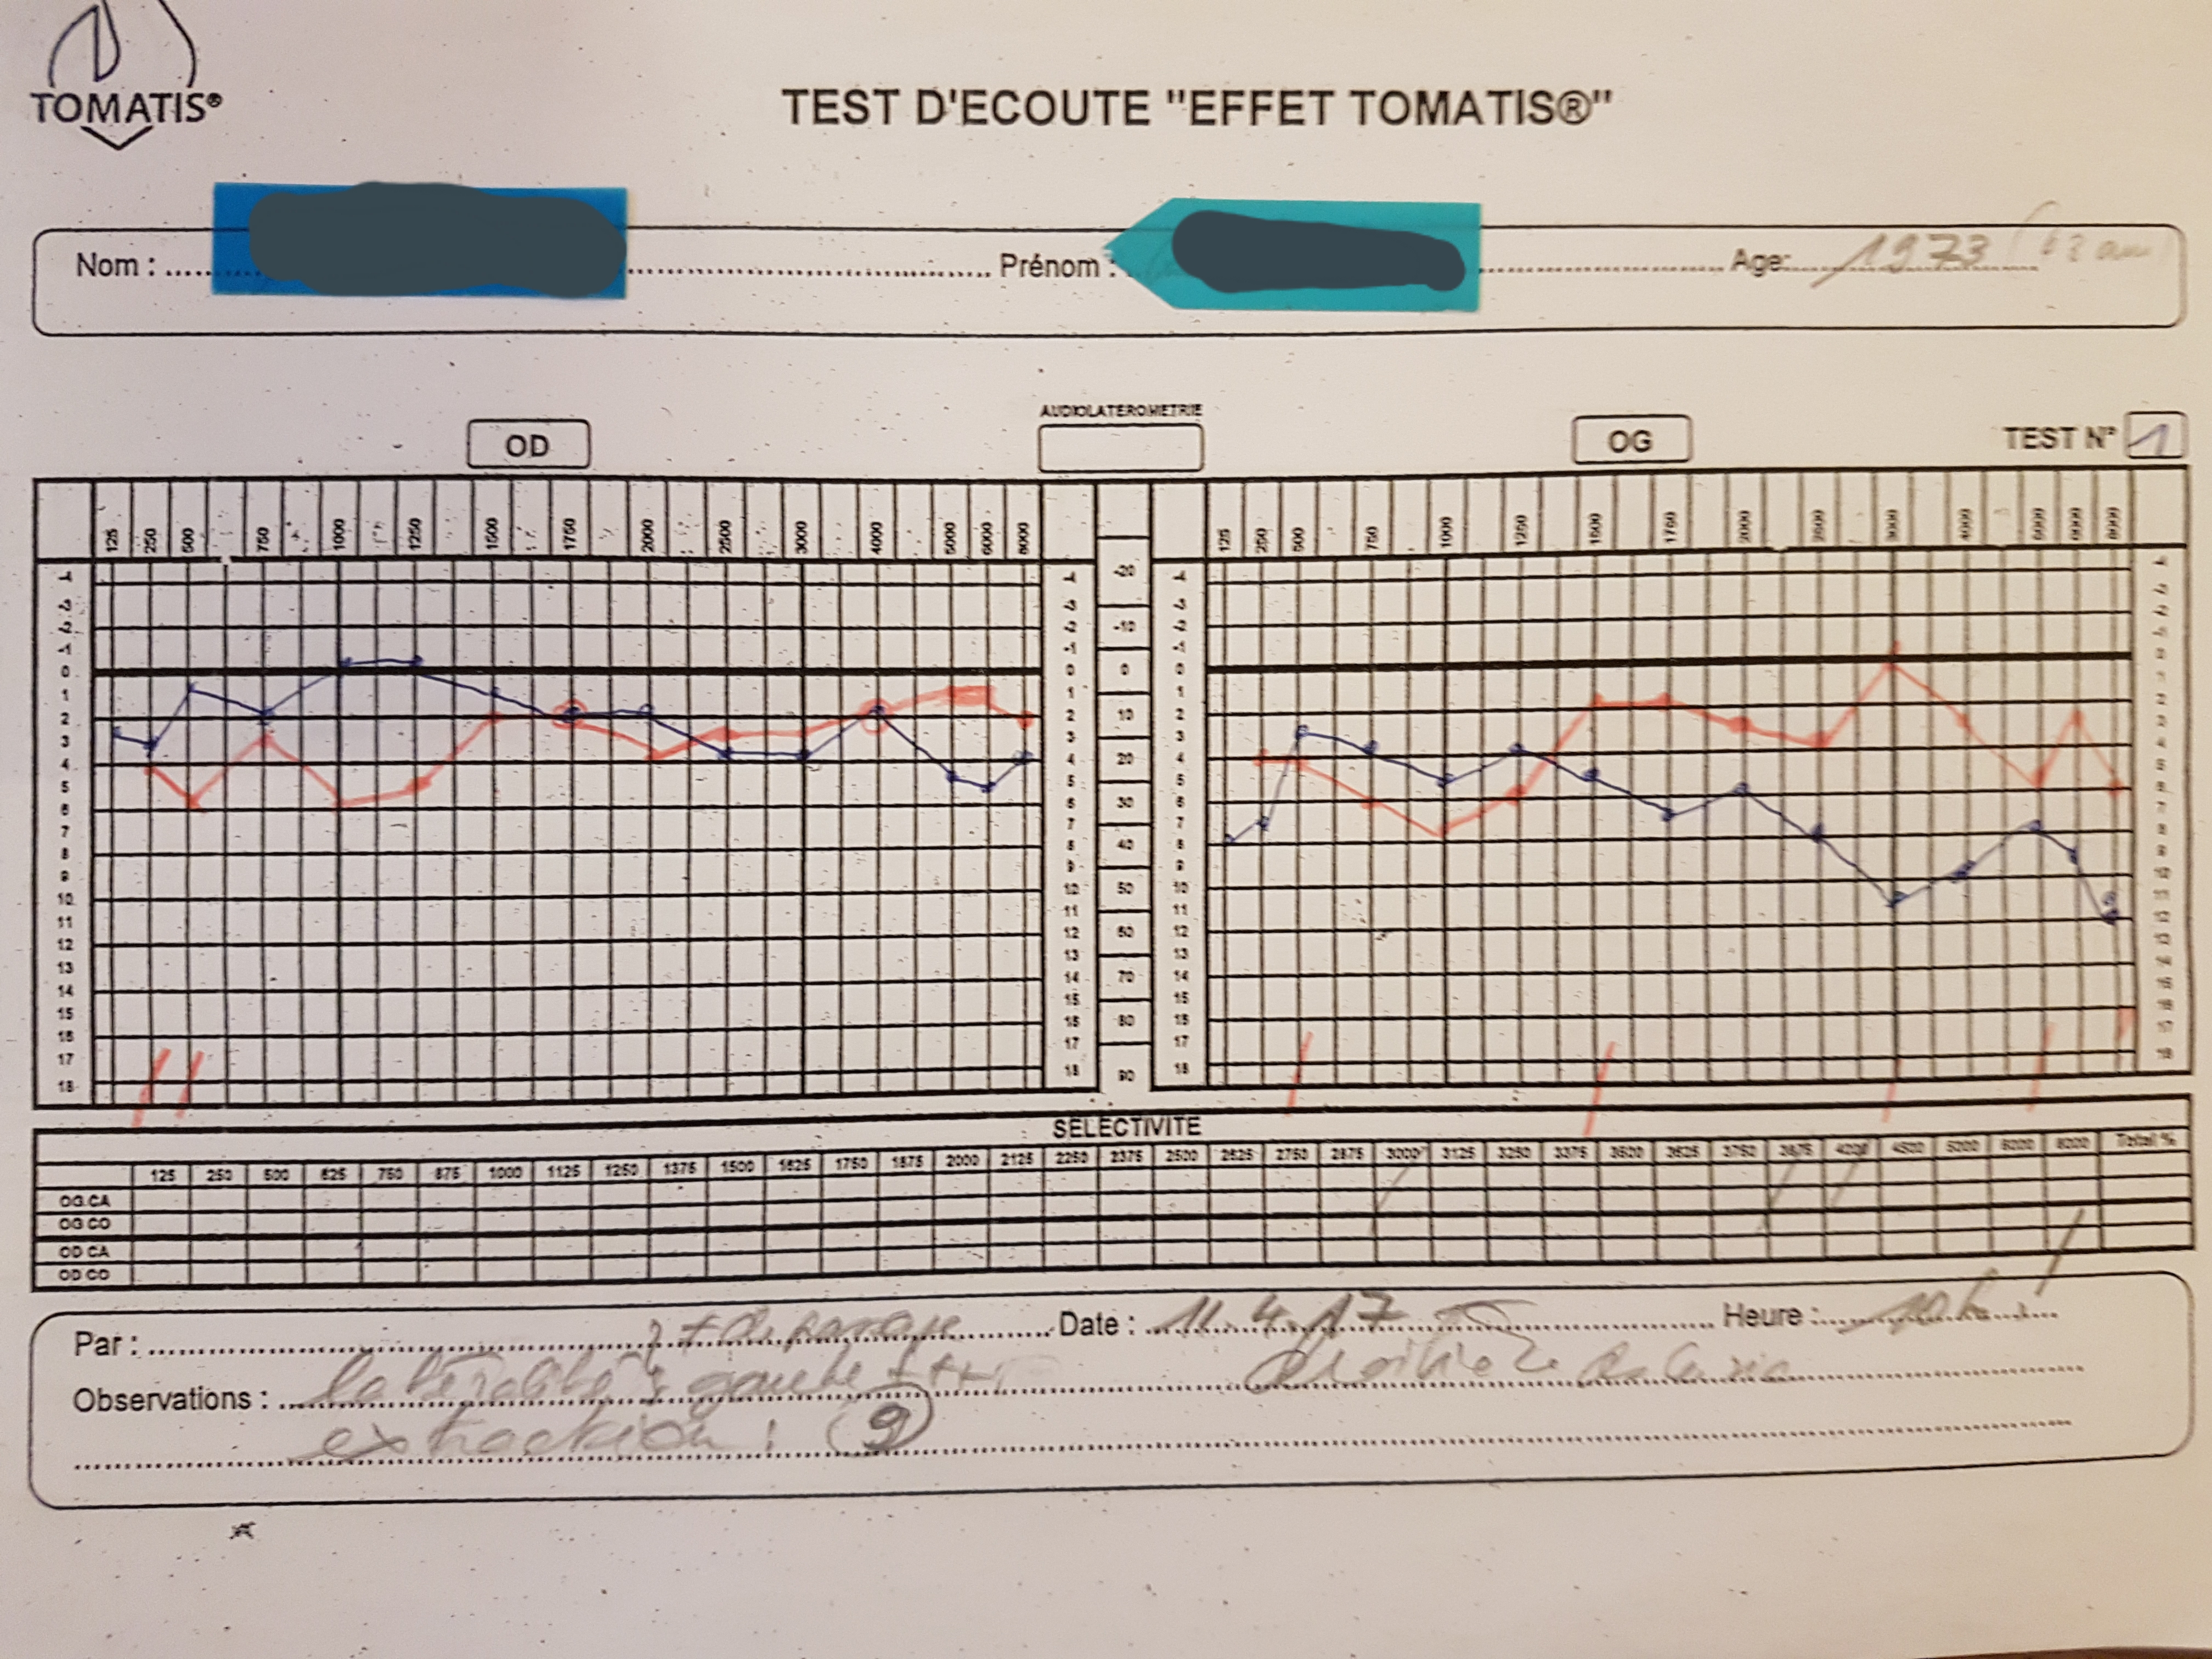
\includegraphics[width=0.7\linewidth]{images/courbesdeepressif.jpg}
	\caption{Courbes caractéristiques du dépressif}
	\label{fig:courbes du dépressif}
      \end{figure}



\subsection{Remarques préalables: }
En vue de la taille réduite des échantillons, il n'est pas
pertinent de se lancer dans une analyse purement
quantitative.

Toutefois, nous 
allons prendre en compte les \textbf{seuils} auditifs, le nombre précis de
\textbf{croisements}, (cf.Zwicker et les distorsions)
 le tout allié à l'observation 
des \textbf{courbes aérienne et osseuse}, 
données relevables sur les
graphiques.
Nous ferons ensuite la corrélation des résultats avec ceux du\textbf{ WHOQOL}.
Enfin, nous ajouterons par un seul exemple d'analyse plus spécifique l'apport des trois zones de fréquences issus des tests d'écoute.

Il s'agira  ainsi d'une étude dite de type  ``aléatoire'' mixant le \textbf{quantitatif  et le qualitatif}.




\section{Résultats et comparaison graphique }
--------------------avant/après de deux tests d'écoute, avec ou sans
  musicothérapie, considérations générales-------------------
Nous allons aborder les résultats obtenus avec les tests d'écoute sur
GM et GC.
Nous avons extrait 3 patients de chaque groupe, nombre réduit, dû au
manque de questionnaires WHOQOL remplis à la fin des séjours, l'objectif
étant d'équilibrer les résultats des deux groupes et de faire une corrélation de ceux-ci avec le questionnaire
WHOQOL.

Nous avons considéré \textbf{ 3 critères} pour chaque groupe, avec comparatif avant/après:
\begin{enumerate}
 \item  moyenne chiffrée des seuils
auditifs de la c.a. et de la c.o. de l'oreille droite et de l'oreille gauche de chaque patient.

\item comparaison graphique des courbes aériennes et osseuses.

\item  nombre de croisements (énumération).
\end{enumerate}

Les \textbf{résultats} se trouvent sous forme de signe mathématique. $+$, $=$, $-$.

Voici leur signification:

$+$   : amélioration, modification;  rapprochement significatif aux courbes dites idéales.

$=$   : peu d'amélioration, correspond à : $+/-$, (si c.a. $ + $ et c.o. $-$, ou vice-versa).

$-$   : pas d'amélioration et pas/très peu  de modification, inversion des courbes (c.o. supérieure à c.a.).

\textbf{Index courbe aérienne et courbe osseuse idéales}:

La moyenne chiffrée de la courbe aérienne: 1,3


La moyenne chiffrée de la courbe osseuse: 3,11

Les \textbf{croisements}:
Moins il y a de croisements, meilleur est le résultat, ce qui correspond à un signe positif : $+$.
Le chiffrage obtenu à partir du test 1° et du test 2° (avant/après) nous permet d'obtenir une comparaison.
Si le chiffre du 2°test est plus petit que le 1°, cela correspond à un signe positif: $+$.
Si le nombre est plus élevé, cela correspond à un signe négatif: $-$.

   
      \subsection{ Comparaison avec les 2 tests d'écoute, moy.or.dr et or.g. pour chaque individu,
       avant/après séjour avec GC et GM:
       }

       \subsubsection{ GC : Résultats détaillés de 3 patients avec les moyennes chiffrées:}



       
      \paragraph{ A. Patient Br.:}
  \begin{figure}
\centering
\includegraphics[width=0.7\linewidth]{images/graphiques/bru_pre.png}
\caption[Moyenne OG+OD]{Premier test Br.}
       
\label{groupecontroleimage1}
\end{figure}

	\begin{enumerate}
 		\item  c.a.: pas de modification, augmentation des
                  seuils: $-$
 		\item  c.o.: redressement des seuils: $+$
 		\item  croisements: $5/4$ : $+$ : ce qui signifie:  5 croisements lors du 1°test// 4 croisements lors du 2° test= nous avons 1 croisement en moins, donc le résultat est considéré comme positif en fin
                  de séjour.
                \end{enumerate}

             \textbf{Conclusion: $- + +   :  =$}
 \begin{figure}
\centering
\includegraphics[width=0.7\linewidth]{images/graphiques/bru_post.png}
\caption[Moyenne OG+OD]{Second test Br.}
       
\label{groupecontroleimage1}
\end{figure}





\paragraph{B. Patient Sch.:}

	\begin{enumerate}
 		
 		\item : c.a.: pas de modification, très légère augmentation des
                  seuils: +/-
 		\item : c.o.: a passé sous c.a., modification des seuils: +
 		\item : croisements: 2/2 :     =
                  
                \end{enumerate}

              \textbf{  Conclusion:  +/-    +    =        :  =}

\begin{figure}
\centering
\includegraphics[width=0.7\linewidth]{images/graphiques/schaff_pre.png}
\caption[Moyenne OG+OD]{Premier test Sch.}
       
\label{groupecontroleimage1}
\end{figure}


         \begin{figure}
\centering
\includegraphics[width=0.7\linewidth]{images/graphiques/schaff_post.png}
\caption[Moyenne OG+OD]{Second test Sch.}
       
\label{groupecontroleimage1}
\end{figure}


\paragraph{C. Patient Wal.:}



\begin{figure}
\centering
\includegraphics[width=0.7\linewidth]{images/graphiques/wal_pre.png}
\caption[Moyenne OG+OD]{Premier test Wal.}
       
\label{groupecontroleimage1}
\end{figure}

	\begin{enumerate}
 		
 		\item : c.a.: peu de modification: =
                
 		\item : c.o.: tentative de rapprochement de c.a. mais
                  reste dominante: -
 		\item : croisements: 1/3 :  -
                  
                \end{enumerate}

                \textbf{ Conclusion:  $= -  -        : -$ }

               \begin{figure}
\centering
\includegraphics[width=0.7\linewidth]{images/graphiques/wal_post.png}
\caption[Moyenne OG+OD]{Second test Wal.}
       
\label{groupecontroleimage1}
\end{figure}
                
  \subsubsection{GM : Résultats détaillés de 4 patients avec les moyennes chiffrées:}

\paragraph{ A. Patient Sw.:}



 \begin{figure}
\centering
\includegraphics[width=0.7\linewidth]{images/graphiques/sw_pre.png}
\caption[Moyenne OG+OD]{Premier test Sw.}
       
\label{groupecontroleimage1}
\end{figure}

	\begin{enumerate}
 		
 		\item : c.a.: pas de modification, 1,27/1,27 : =
                
 		\item : c.o.: redressement et rapprochement, relèvement des seuils, 3,07/3,39: -
 		\item : croisements: 1/3 :  -
                  
                \end{enumerate}

                \textbf{  Conclusion:  = +  -        : ``=''}

                \begin{figure}
\centering
\includegraphics[width=0.7\linewidth]{images/graphiques/sw_post.png}
\caption[Moyenne OG+OD]{Second test Sw.}
       
\label{groupecontroleimage1}
\end{figure}




\paragraph{B. Patient Cav.: }

(pas de WOQOL fin de séjour)


\begin{figure}
\centering
\includegraphics[width=0.7\linewidth]{images/graphiques/cav_pre.png}
\caption[Moyenne OG+OD]{Premier test Cav.}
       
\label{groupecontroleimage1}
\end{figure}

	\begin{enumerate}
 		
 		\item : c.a.: redressement: +
                
 		\item : c.o.: redressement et rapprochement, relèvement des seuils: +
 		\item : croisements: 3/1 :  +
                  
                \end{enumerate}

                \textbf{  Conclusion:  + + +       : ``+''}

                \begin{figure}
\centering
\includegraphics[width=0.7\linewidth]{images/graphiques/cav_post.png}
\caption[Moyenne OG+OD]{Second test Cav.}
       
\label{groupecontroleimage1}
                \end{figure}



                
               \paragraph{ C. Patient M.:}



                \begin{figure}
\centering
\includegraphics[width=0.7\linewidth]{images/graphiques/m_pre.png}
\caption[Moyenne OG+OD]{Premier test M.}
       
\label{groupecontroleimage1}
\end{figure}

	\begin{enumerate}
 		
 		\item : c.a.: redressement:  6,43/6,03: +
                
 		\item : c.o.: redressement et rapprochement, relèvement des seuils: 6,25/5,85:  +
 		\item : croisements: 3/3 :  =
                  
                \end{enumerate}

                \textbf{  Conclusion:  +  +  =     : ``+''}

                        \begin{figure}
\centering
\includegraphics[width=0.7\linewidth]{images/graphiques/m_post.png}
\caption[Moyenne OG+OD]{Second test M.}
       
\label{groupecontroleimage1}
\end{figure}


                
\paragraph{D. Patient K.:}

  (pas de WOQOL fin de séjour)

        \begin{figure}
\centering
\includegraphics[width=0.7\linewidth]{images/graphiques/kad_pre.png}
\caption[Moyenne OG+OD]{Premier test K.}
       
\label{groupecontroleimage1}
\end{figure}
	\begin{enumerate}
 		
 		\item : c.a.: redressement important: +
                
 		\item : c.o.: rapprochement et relèvement des seuils: +
 		\item : croisements: 1/7 :  -
                  
                \end{enumerate}

                \textbf{  Conclusion:  + + -       : ``+''}

                 \begin{figure}
\centering
\includegraphics[width=0.7\linewidth]{images/graphiques/kad_post.png}
\caption[Moyenne OG+OD]{Second test K.}
       
\label{groupecontroleimage1}
\end{figure}
          
\paragraph{ Conclusions générales et résultats:}

             Pour répondre à la question initiale sur l'existence d'une modification du tests d'écoute: Nous nous trouvons
           en présence de deux groupes ayant le même type de
           pathologie avec la constatation suivante: il existe effectivement
          une \textbf{modification de l'écoute avant/après séjour pour les
          deux groupes}.
          Cette modification est nettement plus marquée
          pour GM.
         
          \textbf{GC:  ``=''}

          \textbf{GM: ``+''}

          
          
Les données quantitatives observables dans ces graphiques semblent aller dans le
sens de  l'étude faite par le
CNRS (cf.p.19 J.P.) réalisée à partir des seuils auditifs, à savoir
les patients souffrant de dépression semblent souffrir d'un
appauvrissement caractéristiques de fréquences.


\section{Résultats et comparaison avant/après des questionnaires WHOQOL,
  considérations générales}

Chiffres obtenus à partir des 4
domaines, avant/après séjour avec 3 patients du GC et 2 du GM.
Remarque: plus le chiffre est élevé, meilleur est le score.
\paragraph{ GC Résultats et exemples chiffrés:}



A. Patient Br.:

	\begin{enumerate}
 		\item : 25/27 
 		\item : 21/22
 		\item : 12/11
 		\item : 33/32
                \end{enumerate}
                
        Résultat final: 21,6 contre 23 avant séjour,  ce qui
        correspond au signe négatif: ''-''

        
        B. Patient Sch.:

	\begin{enumerate}
 		\item : 30/27 
 		\item : 20/20
 		\item : 10/10
 		\item : 35/30
         \end{enumerate}
                Résultat final: 21,75 contre 23,75 avant séjour, ce qui
        correspond au signe négatif: ''-''

                
                C. Patient Wal.:
	\begin{enumerate}
 		\item : 24/19
 		\item : 17/18
 		\item : 6/5
 		\item : 27/20
 	\end{enumerate}
        Résultat final: 15,5 contre 18,5 avant séjour, ce qui
        correspond au signe négatif: ''-''

        Conclusion: les résultats sont \textbf{négatifs}, à différents degrés.
        Ces exemples confirment en moyenne 
        le ressenti subjectif de l'ensemble des autres patients GC à la fin de leur séjour.

        \paragraph{GM Résultats chiffrés:}


        
   A. Patient Sw.:
	\begin{enumerate}
 		\item : 26/25 
 		\item : 19/19
 		\item : 8/8
 		\item : 29/30
 	\end{enumerate}
        Résultat final: 20,5 contre 20,5 avant séjour, ce qui
        correspond au signe:  ''=''

        
        B. Patient M.:
	\begin{enumerate}
 		\item : 17/27 
 		\item : 13/23
 		\item : 9/10
 		\item : 24/32
                \end{enumerate}
                 Résultat final: 23 contre 15,75 avant séjour. Signe positif:  ``++''

                 Ainsi,  GM exprime
                 \textbf{positivement }
                 l'ensemble de leur séjour.

               \textbf{ Le schéma de l'ensemble des résultats des
                 questionnaires remplis par les deux groupes se trouvent sous les fig.6.17 et 6.18:}
                
\begin{figure}
\centering
\includegraphics[width=0.7\linewidth]{images/Compcontrole.png}
\caption[Schéma du déroulement]{Comparatif avant/après, 
  WHOQOL, GC}
       
\label{groupecontroleimage1}
\end{figure}

\begin{figure}
\centering
\includegraphics[width=0.7\linewidth]{images/Compmusico.png}
\caption[Schéma du déroulement]{Comparatif  avant/après, WHOQOL, GM.}
       
\label{groupecontroleimage1}
\end{figure}



       \textbf{ Conclusion}: selon les chiffres obtenus, le ressenti
       subjectif d'amélioration psychique 
        des patients suivis en musicothérapie apparait comme
        supérieur.
        De manière générale, l'ensemble des données des deux groupes représentés
        par les graphiques corrobore ce résultat.
        Ces données sont des valeurs indicatives car nous avons conscience que l'échantillonnage ne
        peut pas être représentatif, comme déjà dit plus haut, dû
        notamment à un
        manque de
        questionnaires remplis.
  \paragraph{ Comparaisons des résultats du test et du questionnaire
    réunis avec GC/GM:}


  
  GC:
  \begin{enumerate}
 		\item : test d'écoute: ``='' ou ``+/-''
 		\item : WQ: ``-''
                  
            \end{enumerate}
GM:
  \begin{enumerate}
 		\item : test d'écoute: ``+''
 		\item : WQ: ``+''
                  
               \end{enumerate}

                Il est intéressant de relever l'impact positif de la
                musicothérapie sur GM.
                De plus, le résultat est renforcé et corrélé par celui du WQ.
                

                
                Pour GC, l'ensemble des résultats sont +/- à négatifs.
Il est à remarquer que 
                 \textbf{le test d'écoute a
                apporté des données différentes et complémentaires au
                WQ} : ce peut être une indication de travail, une
              suggestion pour
              solliciter le patient davantage sur différents points
              comme l'extériorisation des sentiments dans l'expression verbale
              (c.a. ne s'étant pas modifiée)
              en constatant, comme ici pour certains patients de GC,  
                l'amorce d'une transformation de l'écoute en
                c.o.. Visiblement, le travail
                thérapeutique devrait être plus diversifié, à plus forte raison avec la musicothérapie, pour aider le
                patient dans sa transformation
               et sa mise en résonance interpersonnelle.
                

     


\subsection{Un cas clinique: Test d'écoute avant musicothérapie}

 	Le patient K.O. souffre de dépression depuis des années. Il se montre très
        intéressé pour participer à l'étude.
 
 	
 	\begin{figure}[tbh]
 		\centering
 		\includegraphics[width=0.7\linewidth]{images/clinique/od_before_meyer.png}
 		\caption{Test d'écoute avant musicothérapie}
 		\label{fig:odbeforemeyer}
 	\end{figure}
 	

	
 	\begin{figure}
 		\centering
 		\includegraphics[width=0.7\linewidth]{images/clinique/comparison_bc_ba_before_vs_ideal_curve_meyer.png}
 		\caption[Comparaison avec la courbe idéale]{Comparaison avant
                  musicothérapie des
                  courbes  avec la courbe idéale}
 		\label{fig:comparisonbcbabeforevsidealcurvemeyer}
 	\end{figure}


	
 	\subsection{Description de deux  séances en musicothérapie}
 	Déroulement général de la 1° séance: 
Ayant le choix devant un grand instrumentarium,
        le patient se dirige spontanément vers le piano et très vite
        l'émotion monte: il pense à son père qui en jouait et qui
        s'énervait contre lui lorsqu'il se mettait  à essayer d'en
        jouer. Il n'a jamais pris de cours, tapote avec un seul doigt et se considère comme
        amusical. Il essaie ensuite l'orgue électrique: les sons bas
        lui procurent un énorme plaisir mais il n'ose pas enfoncer les touches
        complètement car c'est trop fort, dit-il et d'autre part, il craint les
        sons hauts.
        Après un moment,la thérapeute lui suggère d'essayer avec deux doigts.
        Il enclenche le mode ``choeur'' et les sons se font beaucoup
        plus présents, plus forts. Puis il commence à essayer spontanément
        avec les autres doigts et remarque en s'étonnant qu'il se
        dirige tout de même vers les sons
        hauts. Il s'amuse à mêler les différentes tessitures,
        le haut comme le bas.
        Il enclenche le mode ``drums'' et part d'un joyeux
        fou-rire. Retour en enfance, dit-il.
        Il se détend et prend de plus en plus de plaisir à jouer, particulièrement  les sons élevés
        sur la droite et avec la main droite, et fait
        la remarque suivante très surprenante:
        \textit{``Ich kann meine Gefühle mit der rechten Hand steuern!''
        ``Je peux diriger mes sentiments avec ma main droite''.}
 Son expression à ce moment précis de la séance est saisissante: il
        est gaucher et se sent très à l'aise d'utiliser son autre
        main,-- \textit{``Komisch''} -- et c'est un événement complètement nouveau pour lui, une vraie
        découverte--\textit{``Entdeckung''} --.
        Il ajoute de plus que les sentiments avec sa main
        droite ne sont plus une affaire de tête. \textit{``Keine
        Kopfsache mehr'''}. Il expérimente l'inversion des mains pour s'en convaincre et tout redevient comme
        avant, c.à.dire plus dutout fluide et retour au contrôle
        mental, 
        bloquant, dit-il. Il rejoue ensuite comme avant, avec sa main droite et tout
        coule à nouveau, à son plus grand ravissement.
        A la séance suivante, il ressent la nécessité de travailler
        les sons dans tout son corps et choisira le bol tibétain en
        les 
        ressentant intensément: tranquilisation et
        énergie. Il
        exprimera encore sa satisfaction d'utiliser désormais  sa main
        droite qui l'aide, dit-il, à analyser les
        situations et à 
        s'analyser.

      


        
    	\subsection{Test d'écoute après la musicoth.}
 	
 	\begin{figure}[h]
 		\centering

 		\includegraphics[width=0.7\linewidth]{images/clinique/od_after_meyer.png}
 		\caption{Test d'écoute après la musicothérapie}
 		\label{fig:odaftermeyer}
 	\end{figure}
 
  Remarques complémentaires selon les courbes et
  croisements.
  Au niveau de la 3°zone, on remarque un travail remarquable fait dans
  le domaine de la créativité, ce qui fut effectivement le cas avec
  notre patient.
     













        
  \section{La dépression, le burnout et leur expression
    musico--physico--psychologique:}

  
En rapport  avec le chapitre faisant le lien avec la dépression et le
système sensoriel, notamment avec le cortex auditif, nous
avons dressé un portrait
physiologique et psychologique du dépressif 
  en les mettant en correspondance avec les trois zones relevées et
  évoquées plus haut avec quelques remarques sur 
les modifications vocales.
 \paragraph{Essai d'un descriptif du dépressif selon les zones d'nterprétation:}

\begin{itemize}
  	\item Zone 1 :  Le rythme cardiaque: un stress intense va modifier le rythme
  du corps en augmentant ses fréquences. La respiration deviendra
  rapide. Il va s'en suivre une modification des perceptions
  extérieures. Une sensibilité particulièrement accrue aux bruits et
  aux sons peut en découler et être vécue comme une
  atteinte physique et psychique insupportable.
  Le changement de posture et d'attitude corporelle sont
notables (affaissement) et la perte d'énergie physique considérable (épuisement).
	\item Zone 2: La qualité de la voix: changement de la qualité du timbre de la
 voix et de l'émission verbale.	
  La voix se caractérise par son volume, son timbre, sa mélodie et son langage. 
	De manière très appropriées, nous pouvons faire ainsi le
        descriptif général de la voix d'un patient dépressif ou
        stressé avec: le volume, le timbre, la
        mélodie, le langage: 
 	\begin{enumerate}
 		\item le volume : basse intensité, faible dynamique
 		\item la mélodie : monotone, sans modulation
 		\item le timbre : mauvaise qualité due à une pertes des harmoniques
 		\item le langage : difficulté d'élocution, manque de fluidité
 	\end{enumerate}
        Il en découle une communication difficile avec l'entourage qui  conduit au retrait social et à l'enfermement sur soi\footnote{Maryland University, 2004, 168\ieme\ Congrès de la Société
américaine d'acoustique.\autocite{le_service_metronews}. https://www.lci.fr/sante/et-si-on-diagnostiquait-la-depression-avec-u
n-test-vocal-sur-smartphone-1562728.html}.
        
	\item Zone 3: La confusion mentale, la démotivation, la perte d'énergie
psychique, la disharmonie intérieure/extérieure, le non-verbal.
\end{itemize}

 \paragraph{Remarque sur la zone 2 et la "voix" en musicothérapie}
Qu'est-ce que la voix? selon le Larousse, elle est définie comme
l'ensemble des sons produits par les vibrations périodiques des
cordes vocales: celles-ci sont notre principal instrument.
La voix en musicothérapie se révèle être un outil pertinent et délicat
à utiliser. Touchant 
directement 
l'émotion--provoquant un mouvement intérieur--la voix permet d'
éveiller l'affect
et provoque une forte stimulation. Elle n'est amenée que rarement
spontanément par le patient lui-même lors des séances et le thérapeute doit la suggérer
finement.
Ainsi, en supposant que l'audition pose problème dans l'émission
vocale, nous avons une façon différente d'aborder le patient. La
définition de cette
zone de la voix peut permettre de le comprendre différemment dans ses difficultés. 
De même, un analyseur vocal peut permettre de suivre précisément l'amélioration de
l'identité vocale; sa visualisation conforte les progrès grâce aux
formants. L'enveloppe spectrale montre le timbre plus ou moins riche
dans l'empreinte vocale, renseignements précieux selon certaines
difficultés rencontrées par le patient.
  \begin{figure}
	\centering
	\includegraphics[width=0.7\linewidth]{images/courbedepressif.jpg}
	\caption[Exemple d'une courbe de dépressif]{Courbe
          représentative d'un dépressif, extrait de l'étude de Nantes,
         1987.}
       
	\label{groupecontroleimage1}
\end{figure}


\section{Interprétation: les 3 zones de fréquences avec leur résonance en musicothérapie et en
  psychologie}


	\textbf{Informations croisées avec les informations récoltées par les 3 
          zones du test d'écoute:}
          
Les paramètres utilisés en musicothérapie trouvent leur lien avec les
3 zones de fréquences d'interprétation psychologique du test d'écoute.

\begin{itemize}
 \item Le rythme, tempo, puls  =  Z.1: le physique, le corps, l'incorporéisation et
l'intégration du rythme,
la posture d'écoute.

\item La voix, le timbre, la mélodie =  Z.2:  l'expression vocale, la communication,
l'émotionnel, la sensibilité, l'affect.

\item La justesse= l'harmonie (consonance, dissonance) et l'improvisation = Z.3:  la créativité, l'interprétation, la
résonance, la musicalité, la motivation, le non-verbal (
l'intraduisible en mot), l'espace.

\end{itemize}
A cette interprétation graphique, nous pourrions renchérir nos
observations avec les relations
qu'E.
Willems  avait établies entre vie humaine et vie musicale, c.à.dire
\begin{itemize}
  \item vie corporelle (impulsions physiques-----vie rythmique
  \item vie affective (émotions, sentiments)------vie mélodique
    \item vie mentale (raisonnement, intellect-----vie harmonique
\end{itemize}

Si nous référons à la conception antique des chakras ainsi qu'au sens de la
topique de Freud (\textbf{ça, moi et surmoi}), nous trouvons également des correspondances
entre les trois zones de 
fréquences et ``la distribution de l'énergie pulsionnelle'' ou entre
les 
``caractéristiques du son et l'énergie instinctuelles''. \autocite[ch. 13]{auriol:cle} 
``La mélodie est la seule forme musicale de la décharge individuelle, car le rythme est le moteur, pré-musical, et l'harmonie, supra-individuelle `` (Mosonyi, 1935, cité par Michel, 1965).
Pour compléter encore le concept de la zone 3, nous pourrions
également faire un parallèle avec Winnicott et son ``objet
transitionnel'', le jeu , la capacité de créer un espace
intermédiaire par l'invention, la recherche et ce aussi entre le ``le
dehors et le dedans'' tant et si bien que nous serions tentés, et ce n'est qu'une
hypothése, de les relier à l'interprétations de la courbe aérienne et osseuse de Tomatis. 
 
\begin{figure}
	\centering
	\includegraphics[width=0.7\linewidth]{images/testinterpmusico}
	\caption[ L'interprétation des 3 zones et leur correspondance
        en musicothérapie]{Graphique. interprétation des 3 zones du
          test et leur correspondance en musicothérapie}
       
	\label{graphiquecolonnetestmusico}
      \end{figure}


\paragraph{Le corps et le psychisme}

``\emph{l'alliage indissociable du corps et du psychisme, 
visible et lisible, résultat de l'écoute de sons.''}\footnote{\emph{Extrait de l'entretien Tomatis réalisé par Auriol, Anvers 1973}}










      


  
 	
 	
 	
 
       
   
 





      



 











   
 

  

  
  


   
   
   
   







\paragraph{Hypothèse}



\paragraph{Y-a-t-il une modification de l'écoute du patient après une prise
en charge en musicothérapie ?}
Est-ce que le processus d'écoute en musicothérapie améliore la capacité
d'écoute ? Devient-elle différente après une musicothérapie?

Est-ce que les test auditifs avant et après la musicothérapie permettent
de visualiser l'action de la musicothérapie?


\paragraph{Est-ce que les résultats ($=$ un changement dans l'écoute) d'une prise
en charge musicothérapeutique peuvent être lisibles et visibles dans
un test d'écoute?}
Est-ce possible d'évaluer un travail musicothérapeutique au moyen
d'un test d'écoute?
Est-ce que ces résultats sont significatifs? 

\paragraph{Est-ce que l'écoute du patient s'est modifié ? si on a pu observer
une modification, dans quel sens va -t-elle ?}

Le contexte: 
est-ce que le contexte est suffisant pour
ressortir des résultats ?





